% quadrature region in the (E, mucm) plane
\begin{center}
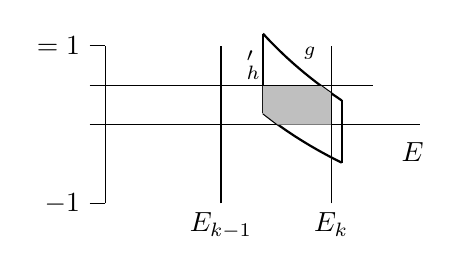
\begin{tikzpicture}
% the axes
  \draw (4.8,0) -- (9, 0);
  \draw (5,-1) -- (5, 1);
% the integration box
  \draw[thick] (7,0.1443) -- (7, 1.1547);
  \draw[thick] (8,-0.4841) -- (8, 0.3067);
% the curves
% Eout: 2
\draw[thick] (7, 0.144338) --
(7.1, 0.0661611) --
(7.2, -0.00780488) --
(7.3, -0.0779271) --
(7.4, -0.144528) --
(7.5, -0.207892) --
(7.6, -0.268272) --
(7.7, -0.325893) --
(7.8, -0.380958) --
(7.9, -0.433646) --
(8, -0.484123);
% Eout: 3
\draw[thick] (7, 1.1547) --
(7.1, 1.04855) --
(7.2, 0.948293) --
(7.3, 0.853396) --
(7.4, 0.763403) --
(7.5, 0.677908) --
(7.6, 0.596552) --
(7.7, 0.519015) --
(7.8, 0.445012) --
(7.9, 0.374288) --
(8, 0.306611);
% integration region
\fill[gray!50] (7, 0.1443) -- (7, 0.5) --
(7.7257, 0.5) -- (7.8, 0.445012) --
(7.86667, 0.3979) -- (7.86667, 0) --
(7.1894, 0) -- cycle;
% data lines
  \draw(4.8,0.5) -- (8.4, 0.5);
  \draw(6.46667, -1) -- (6.46667, 1);
  \node [below] at (6.46667, -1){$E_{k-1}$};
  \draw(7.86667, -1) -- (7.86667, 1);
  \node [below] at (7.86667, -1){$E_k$};
% labels
 \node [below] at (8.9, -0.1){$E$};
 \draw(4.8,-1) -- (5, -1);
 \node [left] at (4.8, -1){$-1$};
 \node [left] at (4.8, 0){$\mucmjm$};
 \node [left] at (4.8, 0.5){$\mucmj$};
  \draw(4.8,1) -- (5, 1);
 \node [left] at (4.8, 1){$\mucm = 1$};
 \node [left] at  (7.1, 0.75){$\calE_h'$};
 \node [above] at  (7.6, 0.7){$\calE_g$};
\end{tikzpicture}
\caption{Integration region of Fig.~\ref{Fig:2-body-region-lab} shown in center-of-mass coordinates}
\label{Fig:2-body-region-cm}
\end{center} 
